\documentclass[11pt,compress,t,notes=noshow]{beamer}\usepackage[]{graphicx}\usepackage[]{color}

\makeatletter
\def\maxwidth{ %
  \ifdim\Gin@nat@width>\linewidth
    \linewidth
  \else
    \Gin@nat@width
  \fi
}
\makeatother

\definecolor{fgcolor}{rgb}{0.345, 0.345, 0.345}
\newcommand{\hlnum}[1]{\textcolor[rgb]{0.686,0.059,0.569}{#1}}%
\newcommand{\hlstr}[1]{\textcolor[rgb]{0.192,0.494,0.8}{#1}}%
\newcommand{\hlcom}[1]{\textcolor[rgb]{0.678,0.584,0.686}{\textit{#1}}}%
\newcommand{\hlopt}[1]{\textcolor[rgb]{0,0,0}{#1}}%
\newcommand{\hlstd}[1]{\textcolor[rgb]{0.345,0.345,0.345}{#1}}%
\newcommand{\hlkwa}[1]{\textcolor[rgb]{0.161,0.373,0.58}{\textbf{#1}}}%
\newcommand{\hlkwb}[1]{\textcolor[rgb]{0.69,0.353,0.396}{#1}}%
\newcommand{\hlkwc}[1]{\textcolor[rgb]{0.333,0.667,0.333}{#1}}%
\newcommand{\hlkwd}[1]{\textcolor[rgb]{0.737,0.353,0.396}{\textbf{#1}}}%
\let\hlipl\hlkwb

\usepackage{framed}
\makeatletter
\newenvironment{kframe}{%
 \def\at@end@of@kframe{}%
 \ifinner\ifhmode%
  \def\at@end@of@kframe{\end{minipage}}%
  \begin{minipage}{\columnwidth}%
 \fi\fi%
 \def\FrameCommand##1{\hskip\@totalleftmargin \hskip-\fboxsep
 \colorbox{shadecolor}{##1}\hskip-\fboxsep
     \hskip-\linewidth \hskip-\@totalleftmargin \hskip\columnwidth}%
 \MakeFramed {\advance\hsize-\width
   \@totalleftmargin\z@ \linewidth\hsize
   \@setminipage}}%
 {\par\unskip\endMakeFramed%
 \at@end@of@kframe}
\makeatother

\definecolor{shadecolor}{rgb}{.97, .97, .97}
\definecolor{messagecolor}{rgb}{0, 0, 0}
\definecolor{warningcolor}{rgb}{1, 0, 1}
\definecolor{errorcolor}{rgb}{1, 0, 0}
\definecolor{code}{rgb}{0.97, 0.96, 1.0}
\newenvironment{knitrout}{}{} % an empty environment to be redefined in TeX

\usepackage{alltt}
\usepackage[utf8]{inputenc}
\usepackage[ngerman]{babel}
\usepackage{dsfont}
\usepackage{verbatim}
\usepackage{amsmath}
\usepackage{amsfonts}
\usepackage{mathtools}
\usepackage{csquotes}
\usepackage{cmbright}
\usepackage{multirow}
\usepackage{longtable}
\usepackage{enumerate}
\usepackage[absolute,overlay]{textpos}
\usepackage{psfrag}
\usepackage{algorithm}
\usepackage{algpseudocode}
\usepackage{eqnarray}
\usepackage{bytefield}
\usepackage{animate}
\usepackage{tikz}
\usetikzlibrary{shapes,matrix,positioning,chains,arrows,shadows,decorations.pathmorphing,fit,backgrounds}
\usepackage{adjustbox}
\usepackage{colortbl}
\usepackage{tabularx} % for tables (incl. \hline)
\usepackage{arydshln} % Load after array, longtable, colortab and/or colortbl , otherwise problems with \hline in tabular env
\usepackage{etex} %increase registers for \dimenS to more than 256, otherwise we get "No room for a new \dimen"
\usepackage{graphicx}
\usepackage{booktabs} %used in epr lectures
\usepackage{bm} % bold greek letters
\usepackage{hyperref} % url citing
\usepackage{blkarray} % block arrays
\usepackage{listings} % block of code
\usepackage{xcolor} %colored math symbols
\usepackage{pgffor}
\usepackage{verbatimbox}
\usepackage{xcolor}

%some colors
\definecolor{checkgreen}{HTML}{18A126}
\definecolor{errorred}{HTML}{FF0000}
\definecolor{blockbg}{HTML}{F7F7F7}
\definecolor{gray}{HTML}{A0A0A0}

% basic latex stuff
\newcommand{\col}{\par\colorbox{code}{\parbox{\textwidth}{\theverbbox}}\par}
\newcommand{\eg}{e.\,g.\xspace} %for example
\newcommand{\ie}{i.\,e.\xspace} %that is to say...
\newcommand{\pkg}[1]{{\fontseries{b}\selectfont #1}} %fontstyle for R packages
\newcommand{\lz}{\vspace{0.5cm}} %vertical space
\newcommand{\oneliner}[1] % Oneliner for important statements
{\begin{block}{}\begin{center}\begin{Large}#1\end{Large}\end{center}\end{block}}
\def\SpAr{\quad \Rightarrow \quad}

%new environments
\newenvironment{vbframe}  %frame with breaks and verbatim
{
 \begin{frame}[containsverbatim,allowframebreaks]
}
{
\end{frame}
}

\newenvironment{vframe}  %frame with verbatim without breaks (to avoid numbering one slided frames)
{
 \begin{frame}[containsverbatim]
}
{
\end{frame}
}

\newenvironment{blocki}[1]   % itemize block
{
 \begin{block}{#1}\begin{itemize}
}
{
\end{itemize}\end{block}
}

\newenvironment{fragileframe}[2]{  %fragile frame with framebreaks
\begin{frame}[allowframebreaks, fragile, environment = fragileframe]
\frametitle{#1}
#2}
{\end{frame}}

\newcommand{\myframe}[2]{  %short for frame with framebreaks
\begin{frame}[allowframebreaks]
\frametitle{#1}
#2
\end{frame}}

\usepackage{../../style/lmu-lecture}

\let\code=\texttt
\let\proglang=\textsf

\setkeys{Gin}{width=0.9\textwidth}

\usepackage{tikz}
\usetikzlibrary{shapes,arrows,snakes, calc}

% Define block styles
\tikzstyle{decision} = [diamond, draw, text width=6em, text badly centered, node distance=4cm, inner sep=0pt]
\tikzstyle{decision2} = [diamond, draw, fill=customgreen!35, text width=6em, text badly centered, node distance=4cm, inner sep=0pt]

\tikzstyle{block} = [rectangle, draw, text width=14em, text centered, rounded corners, node distance=3cm, minimum height=4em]
\tikzstyle{line} = [draw, -latex']
\tikzstyle{cloud} = [draw, ellipse, node distance=3cm, minimum height=2em]

\title{Introduction to Deep Learning}
\author{Bernd Bischl}
\institute{Department of Statistics -- LMU Munich}
\date{WS 2021/2022}

\setbeamertemplate{frametitle}{\expandafter\uppercase\expandafter\insertframetitle}

\IfFileExists{upquote.sty}{\usepackage{upquote}}{}
\input{../../latex-math/basic-math}
\input{../../latex-math/basic-ml}
\input{../../latex-math/ml-nn}

\begin{document}

\lecturechapter{3}{Basic Backpropagation 1}
\lecture{Basic Backpropagation 1}
%%%%%%%%%%%%%%%%%%%%%%%%%%%%%%%%%%%%%%%%%%%%%%%%%%%%%%%%%%%%%%%%%%

\begin{frame}{Backpropagation: Basic Idea}
In DL, we aim to optimize the empirical risk by gradient descent $$\risket = \frac{1}{n} \sumin \Lxyit$$ where $\thetab$ are the weights (and biases) of the network. 

Training of NNs happens in 2 consecutive steps, for one observation $\xb$:
\begin{enumerate}
\item \textbf{Forward pass}: The information of the inputs flow through the model to produce a prediction. Based on that, we compute the empirical loss. We covered that.
\item \textbf{Backward pass / Backpropagation}: The information of the error that happened in the prediction of $\xb$ flows backwards through the model, we calculate the error contribution of each weight to update weights by the negative gradient. 
\end{enumerate}
This is simply gradient descent in disguise (for one observation).
\end{frame}
%%%%%%%%%%%%%%%%%%%%%%%%%%%%%%%%%%%%%%%%%%%%%%%%%%%%%%%%%%%%%%%%%%

\begin{vbframe}{Weight update rule}
  \begin{itemize}
    \item Backpropagation can then be used to compute the gradient of $\Lxyt$ in an \textbf{extremely} efficient way.
    \item The weight update per iteration for one $\xb$ with learning rate $\alpha$, is 
      $$\thetab^{[t+1]} = \thetab^{[t]} - \alpha \cdot \nabla_{\theta}L\left(y, f\left(\xb ~|~ \thetab^{[t]}\right)\right)$$ 
        \item We will see that, at its core, backpropagation is just a clever implementation of the chain rule. Nothing more!

  \item We could now sum up these gradients for all $\xi$ from $\Dset$ to compute the gradient over the complete training set, to perform a full GD step. But as we want to arrive at stochastic gradient descent, 
    we stick for now with updates for a single $\xb$.
  \end{itemize}
\end{vbframe}
%%%%%%%%%%%%%%%%%%%%%%%%%%%%%%%%%%%%%%%%%%%%%%%%%%%%%%%%%%%%%%%%%%


\begin{vbframe}{Backpropagation example}
  \begin{itemize}
    \item Let us recall the XOR example, but this time with randomly initialized weights.
    \item As activations in both the hidden and output layers we apply the \textbf{sigmoidal logistic function}.
    \item To perform one forward and one backward pass we feed our neural network with example $\xb = (1,0)^\top$ (positive sample).
    \item We will optimize the model using the squared error between the binary 0-1 labels and the predicted probabilities instead of the Bernoulli loss. This is
      a bit unusual but computations become simpler for this instructive example.
    \item Then we compute the backward pass and apply backpropagation to update the weights.
    \item Finally we evaluate the model with our updated weights.
  \end{itemize}
\begin{footnotesize}
  Note: We will only show rounded decimals. 
\end{footnotesize}
\framebreak
%%%%%%%%%%%%%%%%%%%%%%%%%%%%%%%%%%%%%%%%%%%%%%%%%%%%%%%%%%%%%%%%%%

  \begin{figure}
    \centering
      \scalebox{0.8}{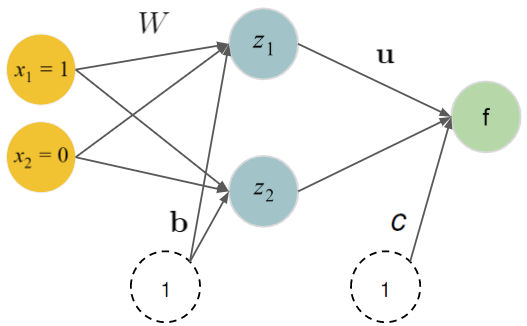
\includegraphics{figure/forwardprop1_new.png}}
      \caption{A neural network with two neurons in the hidden layer. $W$ and $\biasb$ are the weights and biases of the hidden layer. $\wtu$ and $c$ are the weights and bias of the output layer. Based on the values for the weights (and biases), we will perform one forward and one backward pass.}
  \end{figure}
\end{vbframe} 
%%%%%%%%%%%%%%%%%%%%%%%%%%%%%%%%%%%%%%%%%%%%%%%%%%%%%%%%%%%%%%%%%%

\begin{vbframe}{Backprop example: Forward pass}

\begin{itemize}
\item We will divide the forward pass into four steps:
\begin{itemize}
\item the inputs of $z_i$: $\bm{\textcolor{teal}{z_{i,in}}}$
\item the activations of $z_i$: $\bm{\textcolor{teal}{z_{i,out}}}$
\item the input of $f$: $\bm{\textcolor{teal}{f_{in}}}$
\item and finally the activation of $f$: $\bm{\textcolor{teal}{f_{out}}}$
\end{itemize}
\begin{figure}
\centering
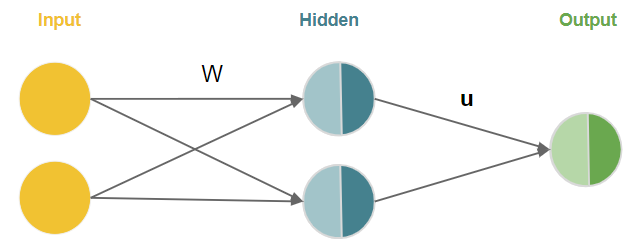
\includegraphics[width=8cm]{figure/xor_rep.png}
\end{figure}
\begin{figure}
\centering
\scalebox{0.5}{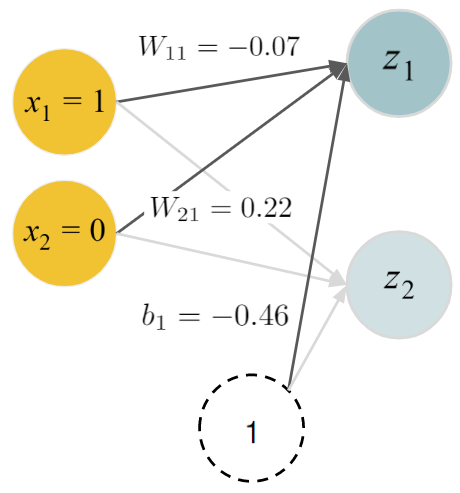
\includegraphics{figure/forwardprop2b_new.png}}
\end{figure}
\begin{footnotesize}
\begin{eqnarray*}
z_{1,in} &=& \Wmat_1^\top \xb + b_1 =  1 \cdot (-0.07) + 0 \cdot 0.22 + 1 \cdot (-0.46) = -0.53 \\
z_{1,out} &=& \sigma\left(z_{1,in}\right) = \frac{1}{1+\exp(-(-0.53))} = \num[round-mode=places,round-precision=4]{0.3705169}
\end{eqnarray*}
\end{footnotesize}
\end{itemize}
\framebreak
%%%%%%%%%%%%%%%%%%%%%%%%%%%%%%%%%%%%%%%%%%%%%%%%%%%%%%%%%%%%%%%%%%

  \begin{figure}
    \centering
      \scalebox{0.5}{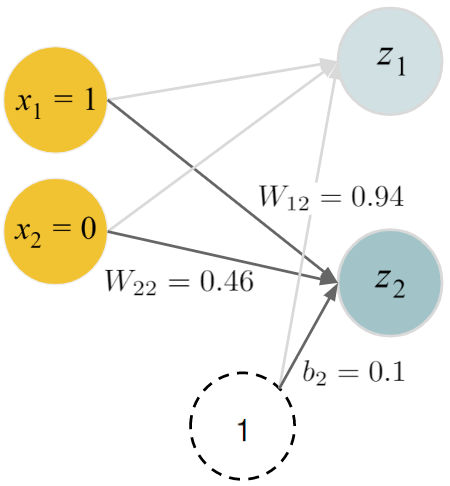
\includegraphics{figure/forwardprop3b_new.png}}
  \end{figure}
\vspace*{-0.5cm}
  \begin{footnotesize}
    \begin{eqnarray*}
    z_{2,in} &=& \Wmat_2^\top \xb + b_2 = 1 \cdot 0.94 + 0 \cdot 0.46 + 1 \cdot 0.1 = 1.04 \\
    z_{2,out} &=& \sigma\left(z_{2,in}\right) = \frac{1}{1+\exp(-1.04)} = \num[round-mode=places,round-precision=4]{0.73885}
    \end{eqnarray*}
  \end{footnotesize}
\framebreak
%%%%%%%%%%%%%%%%%%%%%%%%%%%%%%%%%%%%%%%%%%%%%%%%%%%%%%%%%%%%%%%%%%

  \begin{figure}
    \centering
      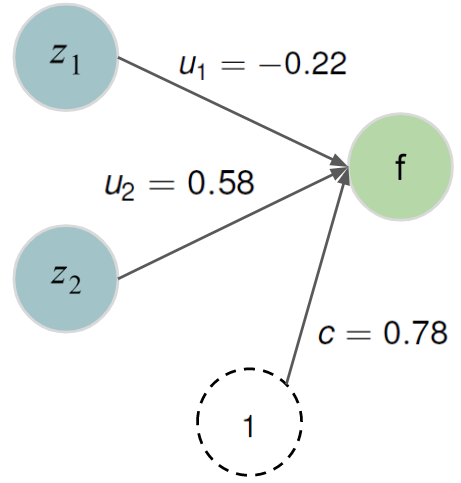
\includegraphics[width=5cm]{figure/forwardprop4b_new.png}
  \end{figure}

\vspace*{-0.5cm}

  \begin{footnotesize}
    \begin{eqnarray*}
    f_{in} &=& \bm{u}^\top \bm{z} + c = \num[round-mode=places,round-precision=4]{0.3705169} \cdot (-0.22) + \num[round-mode=places,round-precision=4]{0.73885} \cdot 0.58 + 1 \cdot 0.78 = \num[round-mode=places,round-precision=4]{1.112242} \\
    f_{out} &=& \tau\left(f_{in}\right) = \frac{1}{1+\exp(\num[round-mode=places,round-precision=4]{-1.112242})} = \num[round-mode=places,round-precision=4]{0.7525469}
    \end{eqnarray*}
  \end{footnotesize}
\framebreak
%%%%%%%%%%%%%%%%%%%%%%%%%%%%%%%%%%%%%%%%%%%%%%%%%%%%%%%%%%%%%%%%%%

  \begin{itemize}
    \item The forward pass of our neural network predicted a value of $$f_{out} = 0.7525$$
    \item Now, we compare the prediction $f_{out} = 0.7525$ and the true label $y = 1$ using the L2-loss: 
      \begin{eqnarray*}
        \Lxy &=& \frac{1}{2}(y - \fxit)^2 = \frac{1}{2}\left(y - f_{out}\right)^{2} \\
                  &=& \frac{1}{2}\left(1 - \num[round-mode=places,round-precision=4]{0.7525469}\right)^2 = \num[round-mode=places,round-precision=4]{0.03061652}
      \end{eqnarray*}
    \item The calculation of the gradient is performed backwards (starting from the output layer), so that results can be reused. 
\end{itemize}
\end{vbframe}
%%%%%%%%%%%%%%%%%%%%%%%%%%%%%%%%%%%%%%%%%%%%%%%%%%%%%%%%%%%%%%%%%%

\begin{vbframe}{Backprop example: Weight Updates}
\begin{itemize}
    \item We will see that the main ingredients to perform the backward pass are: 
    \begin{itemize}
      \item to reuse the results of the forward pass \\ (here:  $\textcolor{teal}{z_{i, in}, z_{i, out}, f_{in},f_{out}}$)
      \item to reuse the \textcolor{violet}{intermediate results} during the backward pass due to the chain rule 
      \item to calculate the derivative of some activation functions and some affine functions
    \end{itemize}
    \item This is demonstrated by continuing the example above.
      \end{itemize}
\framebreak
%%%%%%%%%%%%%%%%%%%%%%%%%%%%%%%%%%%%%%%%%%%%%%%%%%%%%%%%%%%%%%%%%%

  \begin{itemize}
    \item Assume we would like to know how much and in which direction a change in $u_1$ affects the total error. We recursively apply the chain rule and compute: $$\frac{\partial \Lxy}{\partial u_1} = \frac{\partial \Lxy}{\partial f_{out}} \cdot \frac{\partial f_{out}}{\partial f_{in}} \cdot \frac{\partial f_{in}}{\partial u_1}$$
  \end{itemize}
  \begin{figure}
    \centering
      \scalebox{0.54}{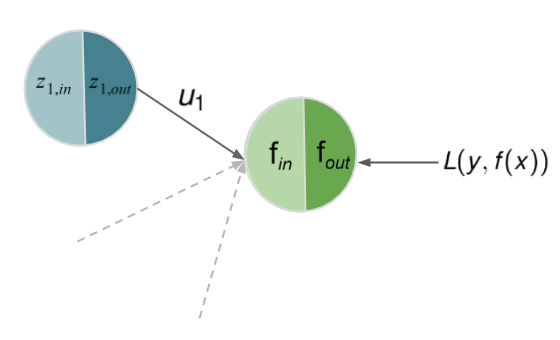
\includegraphics{figure/backprop1_new.png}}
      \caption{\footnotesize{Snippet from our neural network showing the backward path to compute the gradient with respect to weight $u_1$.}}
  \end{figure}
\framebreak
%%%%%%%%%%%%%%%%%%%%%%%%%%%%%%%%%%%%%%%%%%%%%%%%%%%%%%%%%%%%%%%%%%

  \begin{itemize}
    \item 1st step (backwards): We know $\textcolor{teal}{f_{out}}$ from the forward pass.
  \end{itemize}
    \begin{eqnarray*}
      \textcolor{violet}{\frac{\partial \Lxy}{\partial f_{out}}} &=& \frac{d}{\partial f_{out}} \frac{1}{2}(y - f_{out})^2 = -\underbrace{(y - \textcolor{teal}{f_{out}})}_{\hat{=} \text{residual}} \\
       &=& -(1 - \num[round-mode=places,round-precision=4]{0.7525469}) = \num[round-mode=places,round-precision=4]{-0.2474531}
    \end{eqnarray*}
    \begin{figure}
      \centering
        \scalebox{0.6}{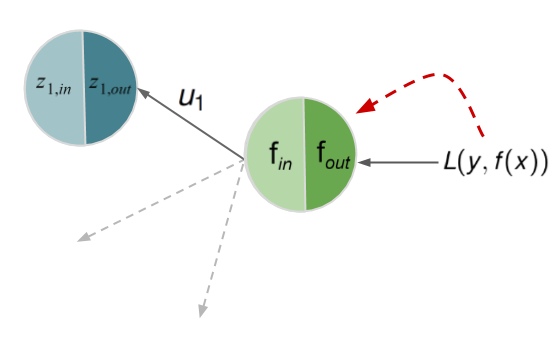
\includegraphics{figure/backprop1_b_new.png}}
        \caption{The first term of our chain rule $\frac{\partial \Lxy}{\partial f_{out}}$}
    \end{figure}
\framebreak
%%%%%%%%%%%%%%%%%%%%%%%%%%%%%%%%%%%%%%%%%%%%%%%%%%%%%%%%%%%%%%%%%%

  \begin{itemize}
    \item 2nd step (backwards). $f_{out} = \sigma(f_{in})$ and we apply the rule for $\sigma'$ (see Chapter 1-3). We already know $\textcolor{teal}{f_{in}}$ from the forward pass.
  \end{itemize}
    \begin{eqnarray*}
      \textcolor{violet}{\frac{\partial f_{out}}{\partial f_{in}}}  &=& \sigma(\textcolor{teal}{f_{in}})\cdot(1-\sigma(\textcolor{teal}{f_{in}})) \\
      &=& \num[round-mode=places,round-precision=4]{0.7525469} \cdot (1 - \num[round-mode=places,round-precision=4]{0.7525469}) = \num[round-mode=places,round-precision=4]{0.1862201}
    \end{eqnarray*}
      \vspace{-0.5cm}
    \begin{figure}
      \centering
        \scalebox{0.6}{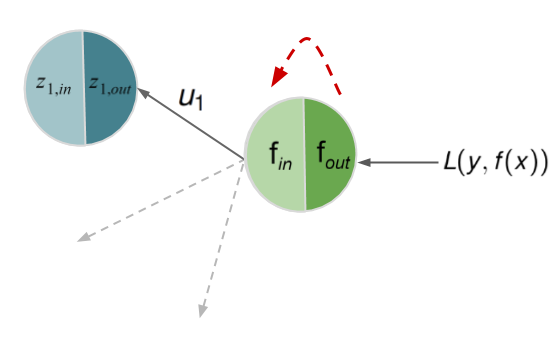
\includegraphics{figure/backprop1_c_new.png}}
        \caption{The second term of our chain rule $\frac{\partial f_{out}}{\partial f_{in}}$}
    \end{figure}
\framebreak
%%%%%%%%%%%%%%%%%%%%%%%%%%%%%%%%%%%%%%%%%%%%%%%%%%%%%%%%%%%%%%%%%%

  \begin{itemize}
    \item 3rd step (backwards).  We know $\textcolor{teal}{z_{1, out}}$ from the forward pass.
  \end{itemize}
    \begin{eqnarray*}
      \textcolor{violet}{\frac{\partial f_{in}}{\partial u_1}} = \frac{\partial (u_1 \cdot z_{1,out} + u_2 \cdot z_{2,out} + c \cdot 1)}{\partial u_1} = \textcolor{teal}{z_{1, out}} = \num[round-mode=places,round-precision=4]{0.3705169}
    \end{eqnarray*}
    \begin{figure}
      \centering
        \scalebox{0.6}{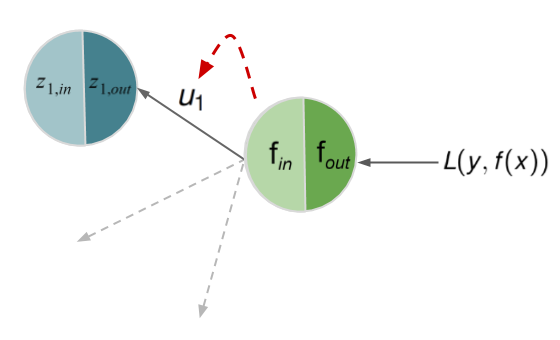
\includegraphics{figure/backprop1_d_new.png}}
        \caption{The third term of our chain rule $\frac{\partial f_{in}}{\partial u_1}$}
    \end{figure}
\framebreak
%%%%%%%%%%%%%%%%%%%%%%%%%%%%%%%%%%%%%%%%%%%%%%%%%%%%%%%%%%%%%%%%%%

  \begin{itemize}
    \item Finally we are able to plug all three parts together and obtain:
  \end{itemize}
  \begin{eqnarray*}
    \textcolor{violet}{\frac{\partial \Lxy}{\partial u_1}} &=& \textcolor{violet}{\frac{\partial \Lxy}{\partial f_{out}}} \cdot \textcolor{violet}{\frac{\partial f_{out}}{\partial f_{in}}} \cdot \textcolor{violet}{\frac{\partial f_{in}}{\partial u_1}} \\
                                        &=& \num[round-mode=places,round-precision=4]{-0.2474531} \cdot \num[round-mode=places,round-precision=4]{0.1862201} \cdot \num[round-mode=places,round-precision=4]{0.3705169} = \num[round-mode=places,round-precision=4]{-0.01707369}
  \end{eqnarray*}
    \begin{figure}
      \centering
        \scalebox{0.6}{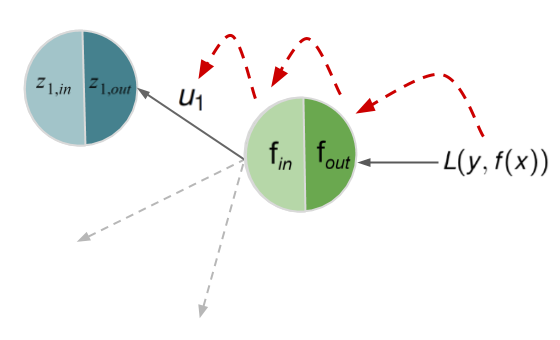
\includegraphics{figure/backprop1_e_new.png}}
        \caption{All three terms of our chain rule $\frac{\partial \Lxy}{\partial u_1} = \frac{\partial \Lxy}{\partial f_{out}} \cdot \frac{\partial f_{out}}{\partial f_{in}} \cdot \frac{\partial f_{in}}{\partial u_1}$}
    \end{figure}
\framebreak
%%%%%%%%%%%%%%%%%%%%%%%%%%%%%%%%%%%%%%%%%%%%%%%%%%%%%%%%%%%%%%%%%%

  \begin{itemize}
    \item Consider a learning rate of $\alpha = 0.5$. Then we obtain:
  \end{itemize}
    \begin{eqnarray*}
      u_1^{[new]} &=& u_1^{[old]} - \alpha \cdot \textcolor{violet}{\frac{\partial \Lxy}{\partial u_1}} \\
                &=& -0.22 - 0.5 \cdot (\num[round-mode=places,round-precision=4]{-0.01707369}) \\
                &=& \num[round-mode=places,round-precision=4]{-0.2114632}
    \end{eqnarray*}
\framebreak
%%%%%%%%%%%%%%%%%%%%%%%%%%%%%%%%%%%%%%%%%%%%%%%%%%%%%%%%%%%%%%%%%%

  \begin{itemize}
    \item We now also want to do the same for $W_{11}$. We have to compute: $$\frac{\partial \Lxy}{\partial W_{11}} = \textcolor{violet}{\frac{\partial \Lxy}{\partial f_{out}}} \cdot \textcolor{violet}{\frac{\partial f_{out}}{\partial f_{in}}} \cdot \frac{\partial f_{in}}{\partial z_{1,out}} \cdot \frac{\partial z_{1,out}}{\partial z_{1,in}} \cdot \frac{\partial z_{1,in}}{\partial W_{11}}$$
  \end{itemize}
  \begin{figure}
    \centering
      \scalebox{0.70}{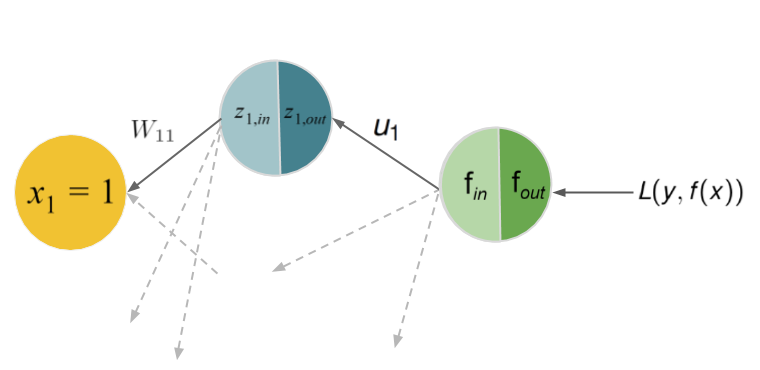
\includegraphics{figure/backprop2_new.png}}
      \caption{Snippet from our neural network showing the backward path to compute the gradient with respect to weight $W_{11}$.}
  \end{figure}
\framebreak
%%%%%%%%%%%%%%%%%%%%%%%%%%%%%%%%%%%%%%%%%%%%%%%%%%%%%%%%%%%%%%%%%%

  \begin{itemize}
    \item We already know $\textcolor{violet}{\frac{\partial \Lxy}{\partial f_{out}}}$ and $\textcolor{violet}{\frac{\partial f_{out}}{\partial f_{in}}}$ from the backward pass before for updating $u_1$.
  \begin{figure}
    \centering
      \scalebox{0.7}{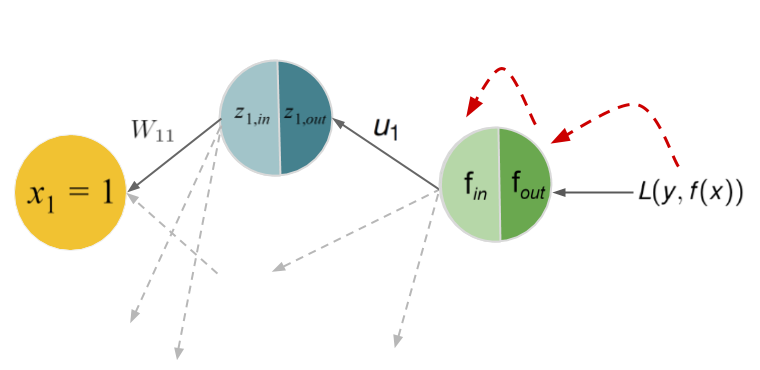
\includegraphics{figure/backprop2_bc_new.png}}
      \caption{The first and second term of our chain rule $\frac{\partial \Lxy}{\partial f_{out}}$ and $\frac{\partial f_{out}}{\partial f_{in}}$}
  \end{figure}
\framebreak
%%%%%%%%%%%%%%%%%%%%%%%%%%%%%%%%%%%%%%%%%%%%%%%%%%%%%%%%%%%%%%%%%%

    \item With $f_{in} = u_1 \cdot z_{1,out} + u_2 \cdot z_{2,out} + c \cdot 1$ we can compute:
  \end{itemize}
  \begin{eqnarray*}
    \textcolor{violet}{\frac{\partial f_{in}}{\partial z_{1,out}}} = u_1 = -0.22
  \end{eqnarray*}
  \begin{figure}
    \centering
      \scalebox{0.7}{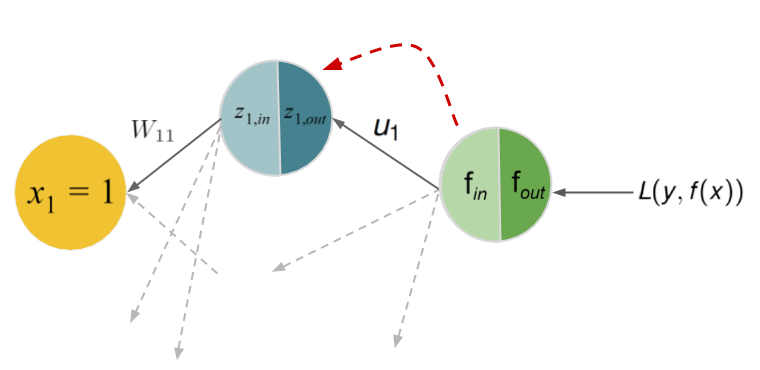
\includegraphics{figure/backprop2_d_new.png}}
      \caption{The third term of our chain rule $\frac{\partial f_{in}}{\partial z_{1,out}}$}
  \end{figure}
\framebreak
%%%%%%%%%%%%%%%%%%%%%%%%%%%%%%%%%%%%%%%%%%%%%%%%%%%%%%%%%%%%%%%%%%

  \begin{itemize}
    \item Next, we need
  \end{itemize}
  \begin{eqnarray*}
    \textcolor{violet}{\frac{\partial z_{1,out}}{\partial z_{1,in}}}  &=& \sigma(\textcolor{teal}{z_{1,in}}) \cdot (1-\sigma(\textcolor{teal}{z_{1,in}})) \\&=&  \num[round-mode=places,round-precision=4]{0.3705169} \cdot (1 - \num[round-mode=places,round-precision=4]{0.3705169}) = \num[round-mode=places,round-precision=4]{0.2332341}
  \end{eqnarray*}
  \begin{figure}
    \centering
      \scalebox{0.7}{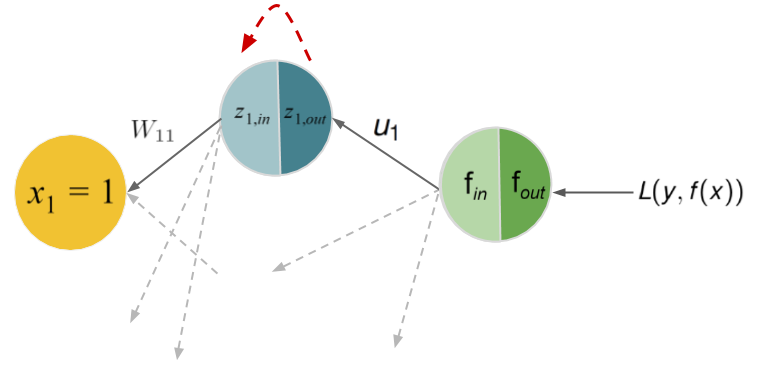
\includegraphics{figure/backprop2_e_new.png}}
      \caption{The fourth term of our chain rule $\frac{\partial z_{1,out}}{\partial z_{1,in}}$}
  \end{figure}
\framebreak
%%%%%%%%%%%%%%%%%%%%%%%%%%%%%%%%%%%%%%%%%%%%%%%%%%%%%%%%%%%%%%%%%%

  \begin{itemize}
    \item With $z_{1,in} = x_1 \cdot W_{11} + x_2 \cdot W_{21} + b_1 \cdot 1$ we can compute the last component:
  \end{itemize}
  \begin{eqnarray*}
    \textcolor{violet}{\frac{\partial z_{1,in}}{\partial W_{11}}} = x_1 = 1
  \end{eqnarray*}
  \begin{figure}
    \centering
      \scalebox{0.65}{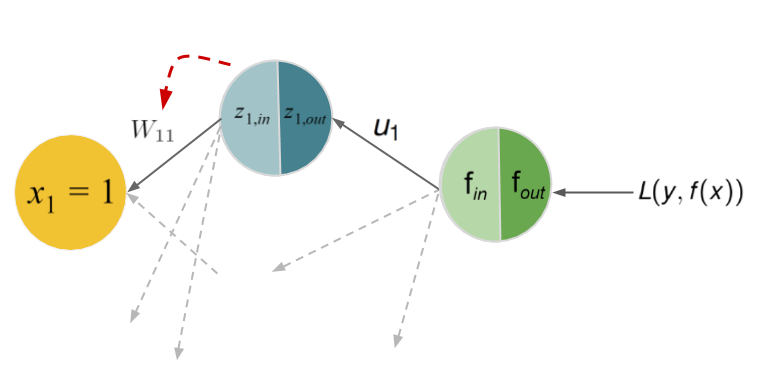
\includegraphics{figure/backprop2_f_new.png}}
      \caption{The fifth term of our chain rule $\frac{\partial z_{1,in}}{\partial W_{11}}$}
  \end{figure}
\framebreak
%%%%%%%%%%%%%%%%%%%%%%%%%%%%%%%%%%%%%%%%%%%%%%%%%%%%%%%%%%%%%%%%%%

  \begin{itemize}
    \item Plugging all five components together yields us: 
      \begin{eqnarray*}
         \textcolor{violet}{\frac{\partial \Lxy}{\partial W_{11}}} &=& 
         \textcolor{violet}{\frac{\partial \Lxy}{\partial f_{out}}} \cdot  \textcolor{violet}{\frac{\partial f_{out}}{\partial f_{in}}} \cdot  \textcolor{violet}{\frac{\partial f_{in}}{\partial z_{1,out}}} \cdot  \textcolor{violet}{\frac{\partial z_{1,out}}{\partial z_{1,in}}} \cdot  \textcolor{violet}{\frac{\partial z_{1,in}}{\partial W_{11}}} 
        \\ &=& (\num[round-mode=places,round-precision=4]{-0.2474531}) \cdot \num[round-mode=places,round-precision=4]{0.1862201} \cdot (-0.22) \cdot \num[round-mode=places,round-precision=4]{0.2332341} \cdot 1 
        \\ &=& \num[round-mode=places,round-precision=4]{0.0023645}
      \end{eqnarray*}
  \begin{figure}
    \centering
      \scalebox{0.6}{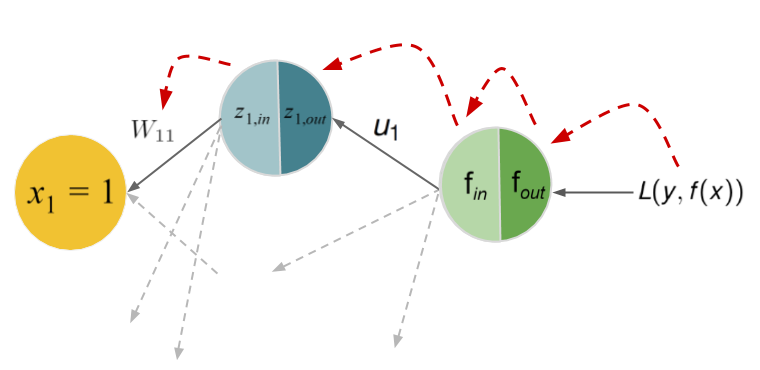
\includegraphics{figure/backprop2_g_new.png}}
      \caption{All five terms of our chain rule}
  \end{figure}
\framebreak
%%%%%%%%%%%%%%%%%%%%%%%%%%%%%%%%%%%%%%%%%%%%%%%%%%%%%%%%%%%%%%%%%%

    \item Consider the same learning rate of $\alpha = 0.5$. Then we obtain:
  \end{itemize}
    \begin{eqnarray*}
      W_{11}^{[new]}  &=& W_{11}^{[old]} - \alpha \cdot  \textcolor{violet}{\frac{\partial \Lxy}{\partial W_{11}}} \\
                  &=& -0.07 - 0.5 \cdot \num[round-mode=places,round-precision=4]{0.0023645} = \num[round-mode=places,round-precision=4]{-0.0711823}
    \end{eqnarray*}
  \begin{itemize}
    \item We would now like to check how the performance has improved. Our updated weights are:
  \end{itemize}
  \begin{eqnarray*}
    W = \begin{pmatrix}
    \num[round-mode=places,round-precision=4]{-0.0711823} & \num[round-mode=places,round-precision=4]{0.9425785} \\
    0.22 & 0.46
    \end{pmatrix},
    b = \begin{pmatrix}
    \num[round-mode=places,round-precision=4]{-0.4611822} \\
    \num[round-mode=places,round-precision=4]{0.1025782}
    \end{pmatrix},
  \end{eqnarray*}
  \begin{eqnarray*}
    u = \begin{pmatrix}
    \num[round-mode=places,round-precision=4]{-0.2114632} \\
    \num[round-mode=places,round-precision=4]{0.5970234}
    \end{pmatrix}
    \text{and} \ c = \num[round-mode=places,round-precision=4]{0.8030404}\text{.}
  \end{eqnarray*}
\framebreak  
%%%%%%%%%%%%%%%%%%%%%%%%%%%%%%%%%%%%%%%%%%%%%%%%%%%%%%%%%%%%%%%%%%

  \begin{itemize}
    \item Plugging all values into our model yields $$f(\xb ~|~\thetab) = \num[round-mode=places,round-precision=4]{0.7614865}$$ and a squared error of $$\Lxy = \frac{1}{2}(1 - \num[round-mode=places,round-precision=4]{0.7614865})^2 = \num[round-mode=places,round-precision=4]{0.02844434}.$$
    \item The initial weights predicted $\fx = \num[round-mode=places,round-precision=4]{0.7525469}$ and a slightly higher error value of $\Lxy = \num[round-mode=places,round-precision=4]{0.03061652}$.
    \lz
    \item Keep in mind that this is the result of only one training iteration. When applying a neural network, one usually conducts thousands of those.
  \end{itemize}
\end{vbframe}
%%%%%%%%%%%%%%%%%%%%%%%%%%%%%%%%%%%%%%%%%%%%%%%%%%%%%%%%%%%%%%%%%%

\begin{frame} {Backpropagation example: Summary}
  \begin{itemize}
    \item Our goal was to minimize the true/expected risk $$\riskt = \E_{(\xb, y)\sim \Pxy} \left[\Lxyt\right]$$
    with respect to the true underlying distribution $\Pxy$.
    \item Because we do not know $\Pxy$, we decided to minimize the empirical risk $$\risket = \frac{1}{n} \sumin \Lxyit$$ w.r.t. the training set and hope for the best.
    \item However, even this is not possible because there is no way to analytically find a global minimum for deep neural networks.
    \item Therefore, we decided to use gradient descent to iteratively find a local minimum of the (typically) non-convex loss function.
  \end{itemize}
\end{frame}
%%%%%%%%%%%%%%%%%%%%%%%%%%%%%%%%%%%%%%%%%%%%%%%%%%%%%%%%%%%%%%%%%%

\begin{frame} {Backpropagation example: Summary}
  \begin{itemize}
      \item To perform gradient descent, we want to compute the gradient of the loss function $\risket$ with respect to \textbf{all} the weights and biases in the network.
      \item Therefore, the number of components in the gradient is the total number of weights and biases in the network.
      \item To compute each component in the gradient, we apply the chain rule to the relevant portion of the computational graph.
      \item In software implementations, a vectorized version of the chain rule is used to compute the derivatives w.r.t. multiple weights simultaneously.
      \item Loosely speaking, each term in the gradient represents the extent to which the corresponding weight is responsible for the loss. In other words, it is a way to assign "blame" to each weight in the network.
  \end{itemize}
\end{frame}
%%%%%%%%%%%%%%%%%%%%%%%%%%%%%%%%%%%%%%%%%%%%%%%%%%%%%%%%%%%%%%%%%%

\begin{vbframe} {Backpropagation example: Summary}

  \begin{itemize}
    \item Gradient descent can be implemented efficiently: 
    \begin{itemize}
      \item We can store and reuse results of the forward pass
      \item We can store and intermediate results due to the chain rule during the backward pass  
      \item We know how derivates of activation functions and affine functions look like
    \end{itemize}
    For example, to compute the derivative of the sigmoid activation at $z_{1,out}$, we \enquote{stored} the derivative of the sigmoid function $\frac{\partial z_{1,out}}{\partial z_{1,in}} = \sigma(z_{1,in})(1-\sigma(z_{1,in}))$ and plugged in $\sigma(z_{1,in}) = \num[round-mode=places,round-precision=4]{0.3705169}$, which was known from the forward pass.
\end{itemize}
\framebreak  
%%%%%%%%%%%%%%%%%%%%%%%%%%%%%%%%%%%%%%%%%%%%%%%%%%%%%%%%%%%%%%%%%%

  \begin{itemize}
  \item In our example, we updated w.r.t. a single training example but typically, we feed subsets of the training set (more on this later).
    \item The term \enquote{backpropagation} refers to the fact that the computation of the gradient using the chain rule is performed backwards (that is, starting at the output layer and finishing at the first hidden layer). 
      A \textbf{forward} computation using the chain rule also results in the same gradient but can be computationally expensive (see http://colah.github.io/posts/2015-08-Backprop/).
 \end{itemize}
\end{vbframe} 
%%%%%%%%%%%%%%%%%%%%%%%%%%%%%%%%%%%%%%%%%%%%%%%%%%%%%%%%%%%%%%%%%%

\begin{frame} {Backpropagation example: Summary}
  \begin{itemize}
    \item After computing the gradient (using backpropagation), we subtract the gradient (scaled by the learning-rate $\alpha$) from the current set of weights (and biases) which results in a new set of weights (and biases).
    \item The empirical loss for this new set of weights is now lower ("walking down the hill").
    \item Next, we once again compute the forward pass for this new set of weights and store the activations.
    \item Then, we compute the gradient of the empirical loss using backpropagation and take another step down the hill.
    \item Rinse and repeat (until the loss stops decreasing substantially). 
      However, we will see later that this naive approach often results in overfitting!
  \end{itemize}
\end{frame}
%%%%%%%%%%%%%%%%%%%%%%%%%%%%%%%%%%%%%%%%%%%%%%%%%%%%%%%%%%%%%%%%%%

\endlecture
\end{document}